\section{Resultados}

O conjunto montado ficou como mostrado na figura \ref{montagem}:

\begin{figure}[h!]
\caption{Montagem do circuito}
\centering % para centralizarmos a figura
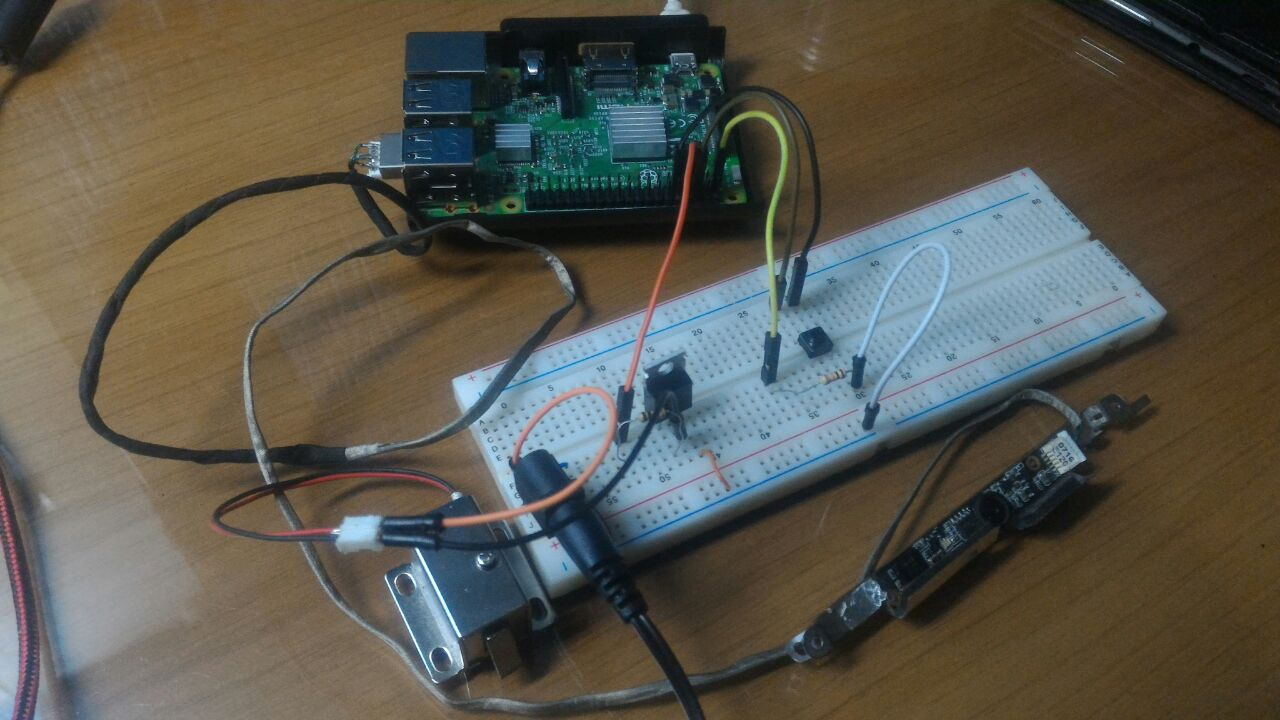
\includegraphics[width=8cm]{montagem.jpeg} % leia abaixo
\label{montagem}
\end{figure}


A ativa��o da trava eletr�nica foi realizada com sucesso, sem sobreaquecimento do transistor, nem falha na comunica��o.

Foi poss�vel comunicar o sistema com o cliente com sucesso, assim como executar os comandos recebidos, como mostram as figuras \ref{terminal} e \ref{terminal2}.

\begin{figure}[h!]
\caption{Cliente liberando porta, porta abrindo com e sem permiss�o}
\centering % para centralizarmos a figura
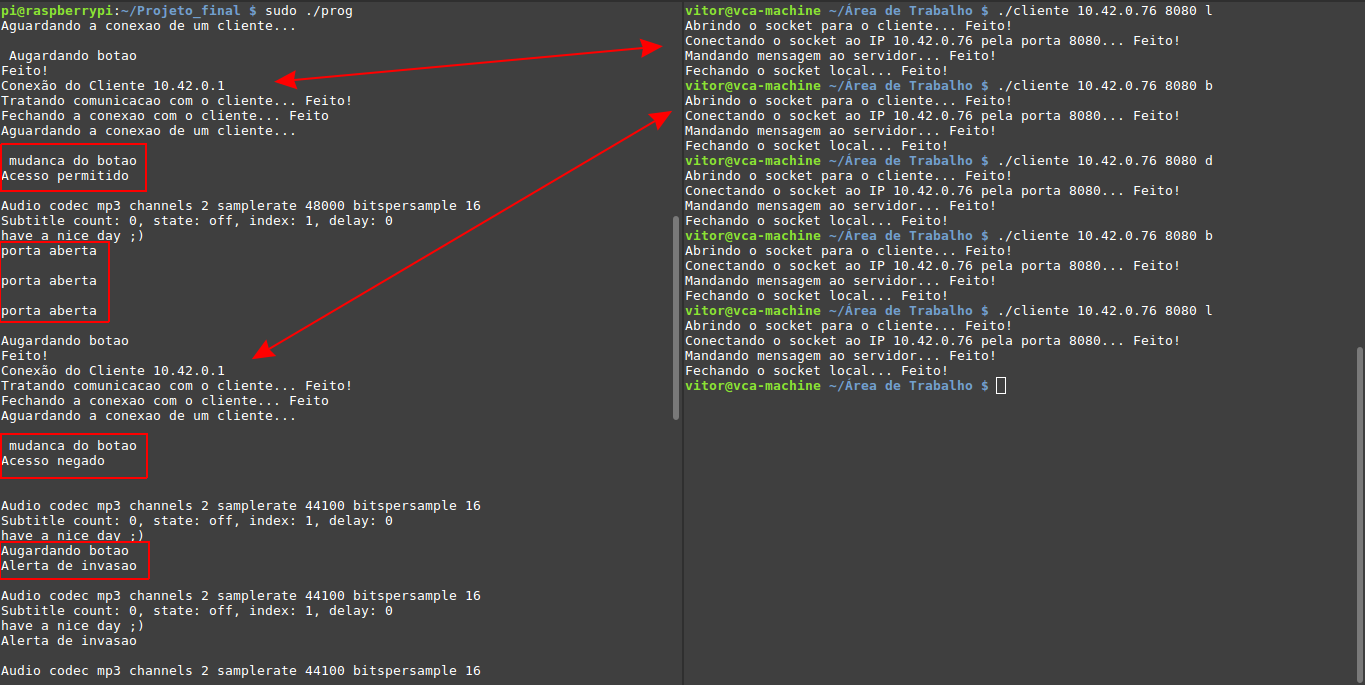
\includegraphics[width=8.5cm]{termin1.png} % leia abaixo
\label{terminal}
\end{figure}

Aqui, o primeiro comando do cliente � para liberar a  entrada. Pode-se observar que o programa s� passa a obedecer novamente quando a porta � fechada. NNa segunda instru��o, o cliente pede que o acesso seja bloqueado. E ent�o ao pressionar o bot�o, o sistema informa "Acesso negado". Ap�s isso foi simulada a abertura da porta por arrombamento, sem que o usu�rio fosse reconhecido. Imediatamente o alerta de invas�o foi ativado.

\begin{figure}[h!]
\caption{Cliente desativando alarme e liberando entrada}
\centering % para centralizarmos a figura
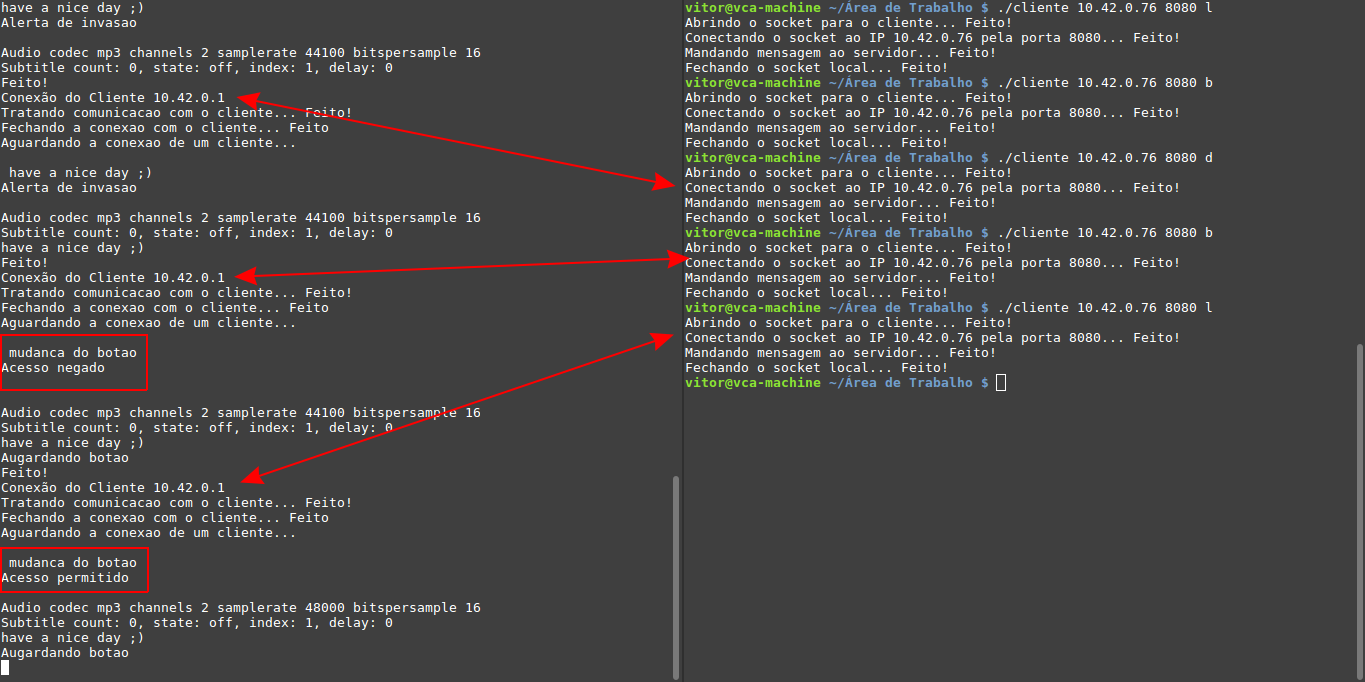
\includegraphics[width=8.5cm]{termin2.png} % leia abaixo
\label{terminal2}
\end{figure}

Aqui, a primeira instru��o do cliente � para desativar o alarme. Ocorrem atrasos at� que o alarme seja completamente desligado. Na segunda instru��o, o cliente bloqueia o acesso e com isso tamb�m ativa o alarme. Ao pressionar o bot�o, o acesso � negado. Ent�o o cliente envia o comando para liberar a porta, e ent�o ao pressionar o bot�o o acesso � liberado.